\chapter{The CMS experiment}
\label{chap:cms}
\chapterquote{All science is either physics or stamp collecting}
{Ernest Rutherford, 1871 -- 1937}

\section{Description}

Brief description of the LHC. Description of the CMS detector with particular focus the ECAL .

\textbf{15 pages}

\section{The LHC}

The \acf{lhc} is an octagonal 27km ring (large) proton-proton (hadron) particle collider. Using a multistage acceleration process two beams of protons are circulated in opposite directions at a centre-of-mass energy, $\sqrt{s}$=7\TeV~(8\TeV) for data collection in 2011 (2012). The beams of protons are accelerated and circulated by electric and magnetic fields respectively. Further precision magnetic fields can control the position and intensity of the beams. There are four points around the ring where the beams can be forced to intersect producing high energy proton-proton collisions. Particle detectors are constructed around these points such that the collision can be reconstructed with the purpose of measuring physical properties and processes, calibration of the detectors with already known processes and searching for new physics. The remainder of this chapter concentrates on a description of one of these detectors, CMS, which the author worked on.

\section{CMS}

The \acf{CMS} detector, pictured in Figure~\ref{fig:cms_diagram}, is a multipurpose experiment designed for the measurement of and search for a multitude of different processes. We will primarily discuss its function as a Higgs finding machine. It has a cylindrical shape consisting of a barrel segment, 21.6m long, and two endcaps, 14.6m in diameter, aligned along the beam direction with its centre at the beam interaction point. The endcaps are those nearer the beam line and so the materials in these components typically have to be able to withstand higher amounts of radiation and therefore tend to have worse performance. Many of its features exploit what one would expect for measuring Higgs decays: it has almost full coverage of the area around the collision point so that nearly every particle emanating from the collision can be reconstructed, it has many complimentary subsystems (or layers) designed to measure different specific particles so that Higgs bosons can be detected through a multitude of decay modes. 

For a Higgs with an intermediate mass (100 - 200 \GeV) the high resolution, (narrow peak) channels, are \HZZ \footnote{A * denotes that one $Z$ can be off-shell} and \Hgg so good energy resolution and identification of electrons and muons is desirable down to very low \pT ($\sim O(10$\GeV) as well as good resolution and identification of high energy photons. 

The central design feature of CMS is the very powerful superconducting magnet which produces an axial magnetic field of 4T. The size of this field, as well as the density of the calorimeter materials, allows for a compact and economical design (much more so than its sister detector, ATLAS). Outside of the magnet lie the muon stations which also serve as a return yoke for the magnetic field. The muon chambers in the barrel consist of alternating layers of drift tubes and restive plate chambers which provide both accurate timing and hit location in order to reconstruct muons down to low energies. In the endcap the drift tubes are replaced with cathode strip chambers. Coupling information from the muon subsystem with information from the inner tracking system allows muons at CMS to \red{insert number here}. The other three main subsystems at CMS, the tracking system and the calorimeters, are located inside the magnetic field.

The first layer is the tracking system which is used to reconstruct the momentum of any outgoing charged particles and to locate the primary and secondary vertices. This is surrounded by the calorimeters, the \acf{ECAL} and the \acf{HCAL}. The first is a single layer of dense, transparent crystals which collects deposits of energy left by electrons and photons which shower inside the material. The second compliments this by providing a measurement of the energy deposited by hadrons (reconstructed as objects known as jets) through nuclear interactions. The \acf{HCAL} is a sampling calorimeter in which the active material (plastic scintillator) is sandwiched between a dense absorbent material. This extends the radiation length of the calorimeter (clearly accommodating the compact design) but degrades the resolution of reconstructing jets. 

\ac{CMS} uses a right-handed Cartesian coordinate system with the origin at the interaction point and the $z$-axis pointing along the beam axis. The $x$-axis points towards the centre of the LHC ring and the $y$-axis points vertically upwards. The azimuthal angle, $\phi \in [-\pi,\pi]$, is defined with respect to the $x$-axis in the transverse $(x-y)$ plane. The polar angle $\theta$ is measured from the $z$-axis. Commonly, the direction of an outgoing particle is defined by $\phi$ and its pseudo-rapidity $\eta$,

\begin{equation}
	\eta = -\ln\tan\biggl(\frac{\theta}{2}\biggr).
\end{equation}

The LHC is capable of producing 40M bunch collisions per second although many of these are not hard interactions, the result being that the outgoing particle debris follows the beam line. A hard (and therefore interesting) collision is characterised by the amount of energy produced in the transverse ($x-y$) plane. Therefore particles are commonly characterised by the projection of their momentum onto this plane, their transverse momentum,

\begin{equation}
	p_{T} = \sqrt{p_{x}^{2}+p_{y}^{2}},
\end{equation}

and the corresponding transverse energy, $E_{T} = E\sin(\theta)$.

\begin{figure}
  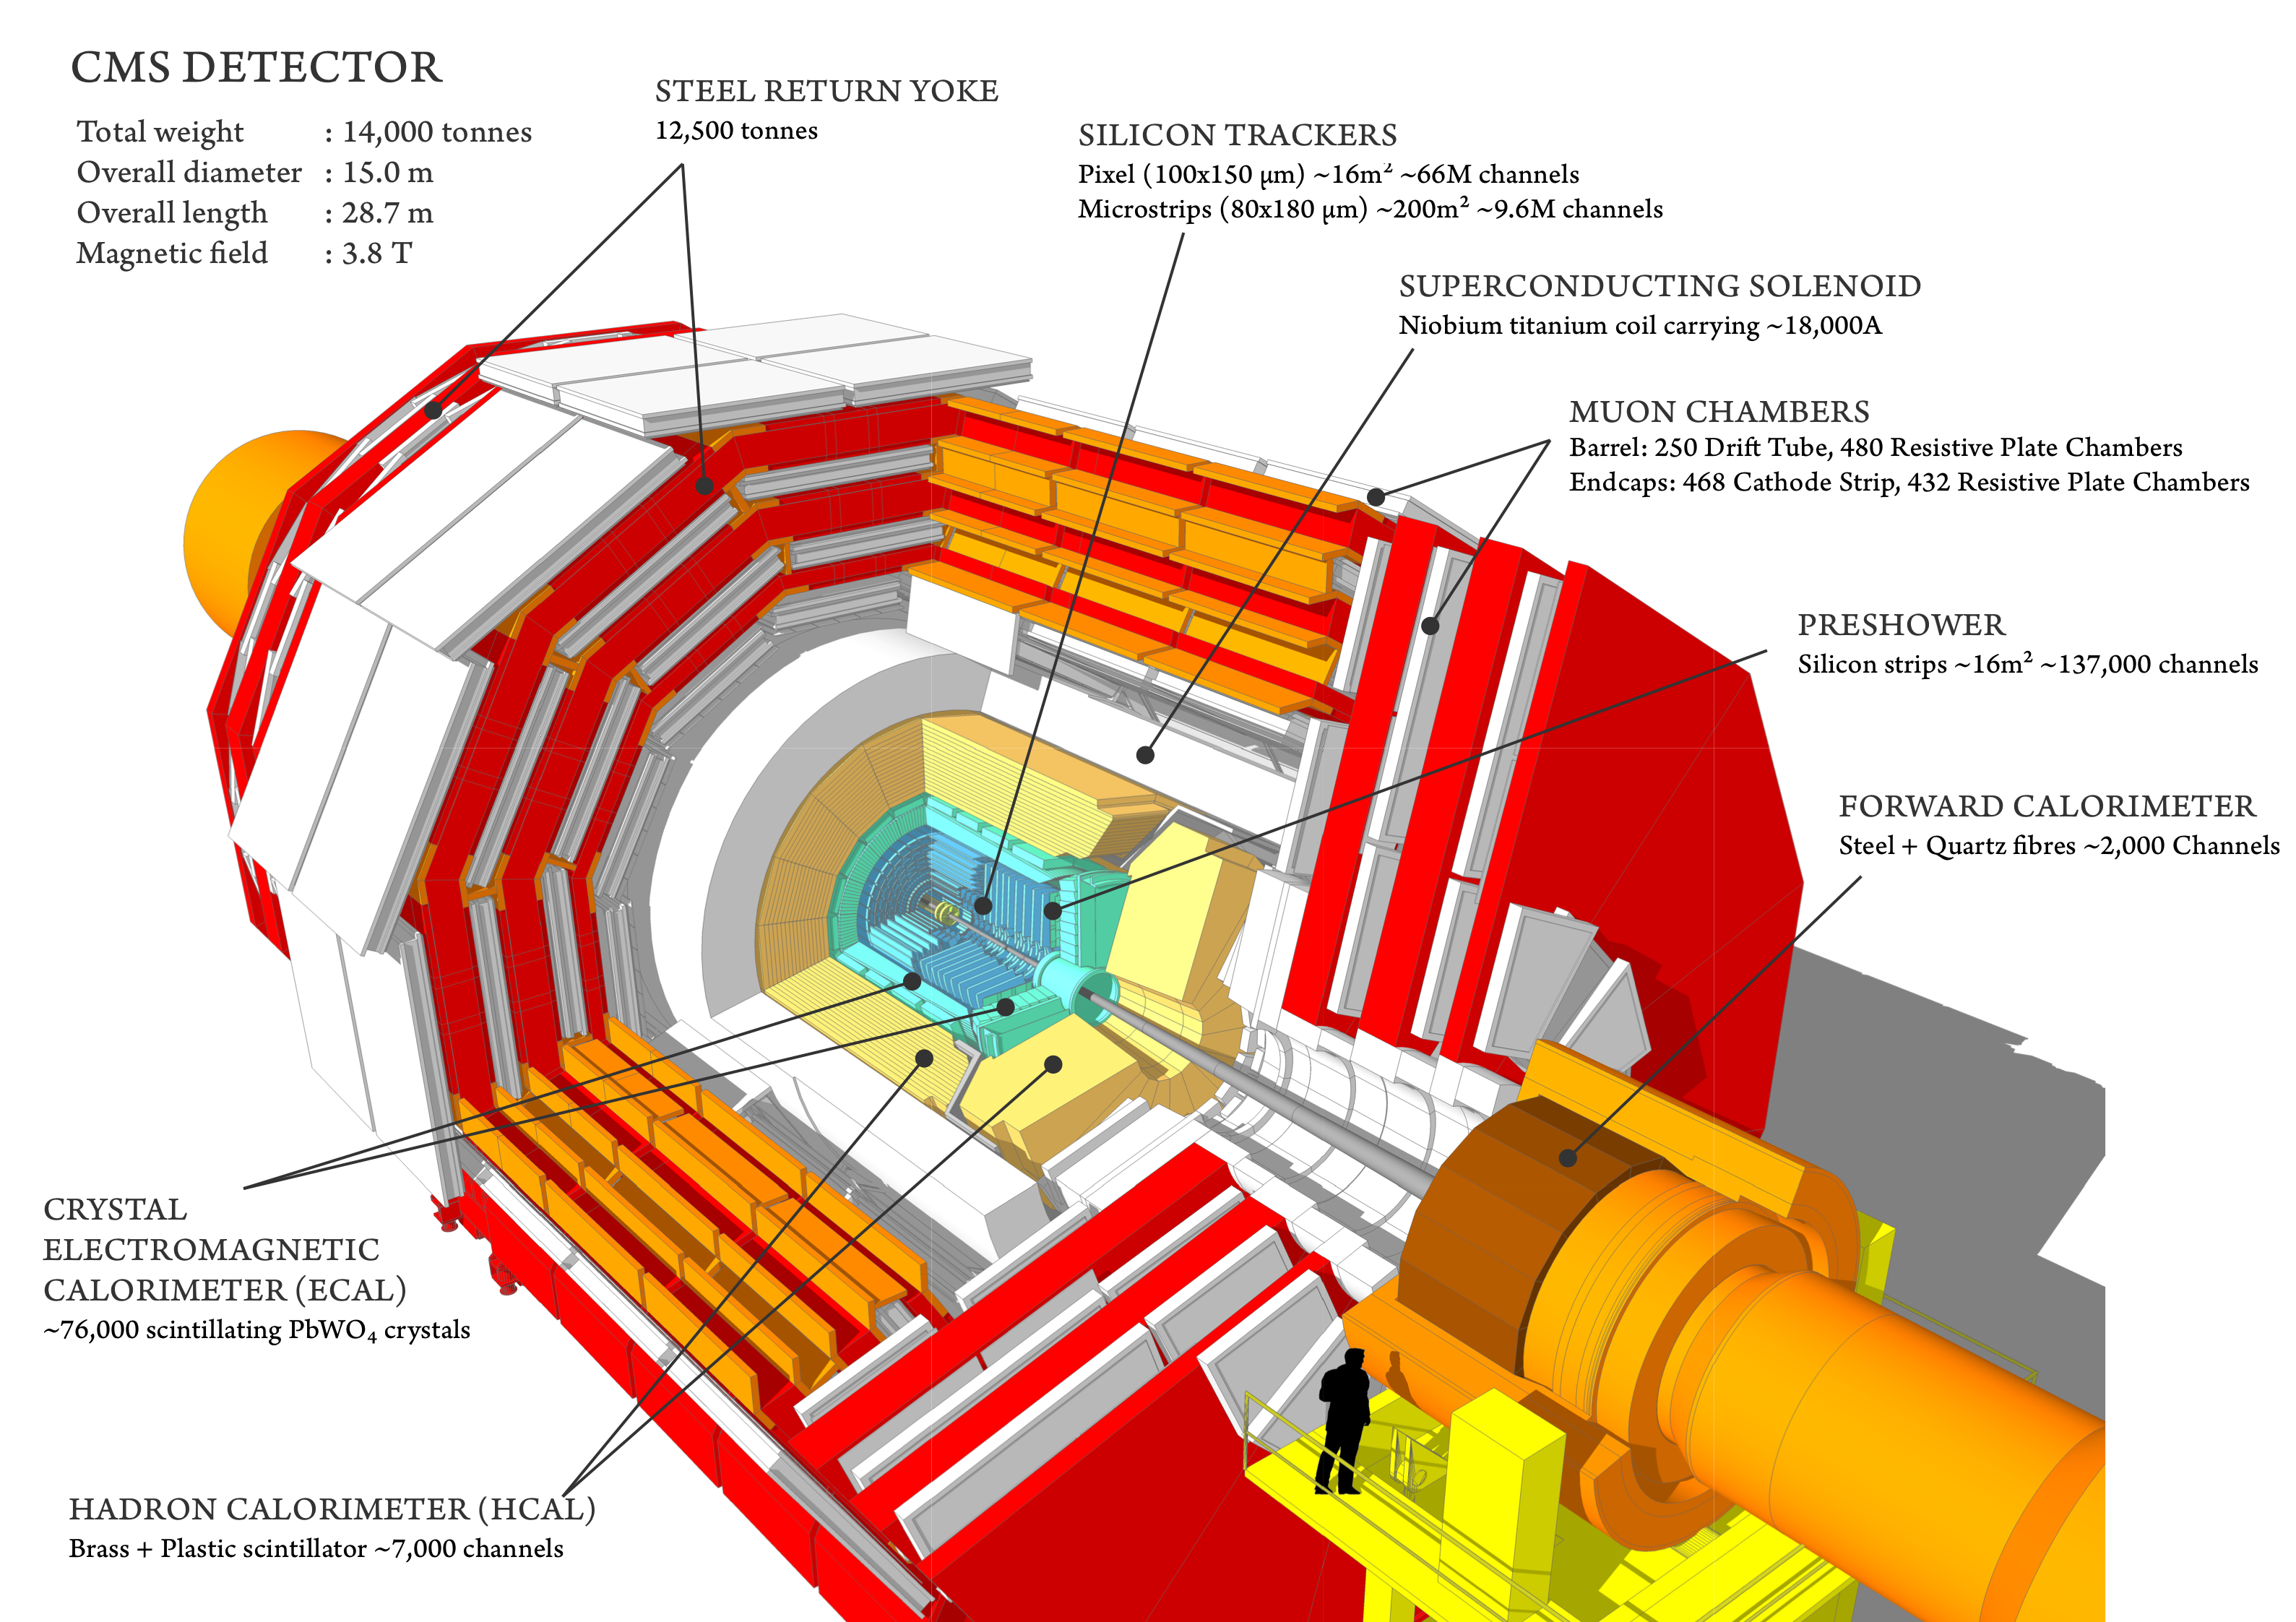
\includegraphics[width=0.8\textwidth]{ch2_cms_exp/plots/cms_diagram.png}
  \caption[CMS diagram]{This is a schematic representation of \ac{cms}}
  \label{fig:cms_diagram}
\end{figure}

\subsection{Tracking system}



\subsection{ECAL}

\subsubsection{Material description}

\subsubsection{Photon reconstruction}
- super cluster algorithm
- differences between photons and electrons (hence why so good for comparisons because can ignore the electron track)

\subsubsection{Photon corrections}
- photon resolution formula
- transparency corrections
- crack corrections etc. (superseding by regression)

\subsection{HCAL}

\subsection{Muons}

\subsection{Isolation and particle flow}





